\documentclass{article}
\usepackage{spconf,amsmath,amssymb,graphicx,booktabs,url}
\usepackage{xeCJK,etoolbox}
\renewcommand{\abstract}{\begin{center}\textbf{摘要}\vspace{-.5em}\end{center}}
\renewcommand{\keywords}{\vspace{.5em}\textbf{关键词}\quad}
\patchcmd{\thebibliography}{\section{References}}{\section{参考文献}}{}{}
\makeatletter
\renewcommand{\fnum@figure}{\textbf{图~\thefigure}}
\renewcommand{\fnum@table}{\textbf{表~\thetable}}
\makeatother
\setCJKmainfont{SimSun}[AutoFakeBold=true,ItalicFont=KaiTi]
\setCJKsansfont{SimHei}
% Verified values generated from the paused snapshots.
\newcommand{\BaseBest}{0.025080}
\newcommand{\BaseEnd}{0.025618}
\newcommand{\BridgeBest}{0.024445}
\newcommand{\BridgeEnd}{0.028603}
\newcommand{\BridgeBestGain}{2.53}
\newcommand{\BridgeEndHarm}{11.65}
\newcommand{\SensorBestGain}{1.36}
\newcommand{\SensorEndHarm}{1.21}
\newcommand{\BridgeSSIM}{0.93509}
\newcommand{\BaseSSIM}{0.93878}
\newcommand{\BridgePatchWins}{63}
\newcommand{\BridgeDiff}{0.635}
\newcommand{\BridgeLower}{-0.005}
\newcommand{\BridgeUpper}{1.256}
\newcommand{\BridgeLow}{+7.71}
\newcommand{\BridgeMid}{+5.39}
\newcommand{\BridgeHigh}{-5.19}
\newcommand{\BridgeExtraParams}{9,223}

\newcommand{\StageResultRows}{%
Base & 0.025618 & 32 & 0.025080 & \textemdash & 0.93878 & 0.08987 & 1.0701 & 0.82951 \\
I02 & 0.028603 & 9 & 0.024445 & +2.53 & 0.93509 & 0.08641 & 0.9715 & 0.82545 \\
I01 & 0.025929 & 22 & 0.024740 & +1.36 & 0.94123 & 0.08470 & 1.0037 & 0.82605 \\
I06 & 0.026038 & 32 & 0.025230 & -0.60 & 0.93716 & 0.08892 & 1.0811 & 0.82428 \\
I03 & 0.025477 & 38 & 0.025350 & -1.07 & 0.93865 & 0.09061 & 1.0832 & 0.82415 \\
I05 & 0.026412 & 24 & 0.025371 & -1.16 & 0.93863 & 0.08789 & 1.0560 & 0.82452 \\
I07 & 0.026729 & 18 & 0.025494 & -1.65 & 0.93504 & 0.08966 & 1.0870 & 0.82551 \\
I13 & 0.026042 & 32 & 0.025517 & -1.74 & 0.93904 & 0.08903 & 1.0535 & 0.81914 \\
}

\graphicspath{{figures/}}
\newcommand{\obs}{\mathcal{O}}
\newcommand{\target}{F^\star}
\title{面向单步遥感时空融合的双锚条件扩散桥}
\name{匿名作者}
\address{阶段定稿，2026 年 11 月 22 日}

\begin{document}
\ninept
\maketitle

\begin{abstract}
单步时空融合只调用一次去噪主干，利用粗观测与精细参考重建目标日精细影像。本文考察初始噪声状态对重建的影响，构造一种双锚条件扩散桥。该模型按采集间隔构造均值先验，并用同一组观测预测空间变化的噪声尺度。在 Lower Gwydir Catchment（LGC）开发验证集上，按验证 RMSE 选择检查点后，双锚扩散桥将平均 patch RMSE 从 \BaseBest{} 降至 \BridgeBest{}，相对下降 \BridgeBestGain\%。统一取第 40 轮时，RMSE 从 \BaseEnd{} 升至 \BridgeEnd{}。按粗观测相对参考插值的偏离程度分层后，低偏离组的误差下降，最高组的误差升高。上述观测来自一个训练种子和一个验证日期，说明检查点选择与粗观测时间偏离是评价该扩散桥时需要控制的条件。
\end{abstract}

\begin{keywords}
时空融合, 遥感, 扩散桥, 双锚, 验证轨迹
\end{keywords}

\section{引言}
高空间分辨率卫星影像往往难以兼顾密集的时间覆盖。双锚时空融合使用目标日前后的两幅精细影像和三幅粗观测，估计缺失的目标日精细影像。粗观测提供目标日的变化线索，两幅精细参考提供空间结构。参考结构的位置与外观也可能随时间改变。

STFDiff 等条件扩散模型将这些观测用于去噪~\cite{huang2024stfdiff}。单次去噪可压缩重建的调用预算~\cite{song2021ddim}。在本文采用的本地单步基线中，去噪状态从标准高斯噪声出发，而两幅精细参考通过条件分支进入主干。本文检验可观测数据构建的初始分布能否在相同主干调用次数下改善重建，并考察收益能否保持到共同训练终点。

本文在共享的 STFDiff 主干上实现双锚扩散桥，将按日期加权的精细参考、可学习残差与空间噪声尺度用于构建初始状态（图~\ref{fig:bridge}）。本次分析覆盖已经完成的八组训练，报告共同终点与最佳检查点，按粗观测时间偏离程度比较逐块收益。另保留在去噪后施加传感器算子的一组独立对照。

\section{相关工作}
STFDiff 从历史观测学习精细影像的条件分布~\cite{huang2024stfdiff}。SA-STF 将时间特征对齐、语义自适应融合与残差扩散结合~\cite{zhang2026sastf}。近期的图像恢复工作用空间不确定性引导扩散桥~\cite{tu2026udbm}。遥感领域的 WPFM-STF 则采用小波约束和流匹配，将学习的时空先验输运至目标~\cite{hu2026wpfm}。本文固定五观测输入和去噪主干，考察按采集日期加权的双锚先验和高斯噪声尺度在训练加噪与单步推理起点中的作用。

\section{方法}
\subsection{观测协议}
以 $\obs=(F_-,F_+,C_-,C_0,C_+)$ 表示较早与较晚的精细参考、对应日期的粗观测和目标日粗观测 $C_0$。各观测在共同网格上对齐，每块大小为 $256\times256$，包含六个波段。模型输入缩放至 $[-1,1]$，评价时恢复到反射率域。目标精细影像记作 $\target$，用于训练加噪和损失计算，并作为评价参照。

\subsection{双锚初始分布}
令 $\Delta_-$、$\Delta_+$ 分别为前锚至目标日、目标日至后锚的天数，时间权重为 $w=\Delta_-/(\Delta_-+\Delta_+)$。先验头 $G$ 接收拼接后的 30 通道观测，输出七张图 $q=G(\obs)$。先验头由 $3\times3$ 卷积、逐通道 $3\times3$ 卷积及 $1\times1$ 投影组成，前两层宽度为 32。均值与尺度写作
\begin{align}
P&=(1-w)F_-+wF_++0.2\tanh(q_{1:6}),\\
s&=0.05+0.45\,\mathrm{sigmoid}(q_7).
\end{align}
$P$ 具有六个波段。$s$ 为六波段共享的逐像素尺度图。采集间隔决定前后锚融合权重，先验头从五幅观测提取残差与尺度。

训练使用 100 级余弦噪声计划 $\bar\alpha_k$，构造扰动影像
\begin{equation}
X_k=P+\sqrt{\bar\alpha_k}(\target-P)
       +\sqrt{1-\bar\alpha_k}\,s\varepsilon,\quad
\varepsilon\sim\mathcal{N}(0,I),
\label{eq:bridge}
\end{equation}
其中 $k\in\{0,\ldots,99\}$。双流去噪器 $D_\theta$ 分别编码 $\obs$ 和 $X_k$，结合残差特征与噪声时间条件预测精细影像，将输出截断到 $[-1,1]$。损失为 $\operatorname{MAE}(\widehat{F},\target)+\mathcal{L}_{P,s}$，其中
\begin{align}
\mathcal{L}_{P,s}={}&0.1\left\langle |P-\target|\right\rangle\\
&+0.005\left\langle
\frac{(P-\target)^2}{s^2+10^{-6}}+2\log s\right\rangle .
\end{align}
尖括号表示对像素和波段求均值。最后一项按预测尺度加权先验残差。尺度图能否给出校准的不确定性仍需独立评价。

推理时用 $X_{99}=P+s\varepsilon$ 初始化，只调用一次 $D_\theta(\obs,X_{99},99)$ 得到截断后的预测。基础模型取 $P=0$、$s=1$，省去先验辅助损失。两种配置的去噪主干均调用一次。双锚扩散桥在基础模型 7,488,966 个参数上增加 \BridgeExtraParams{} 个参数，并额外调用一次先验头。

\begin{figure*}[t]
\centering
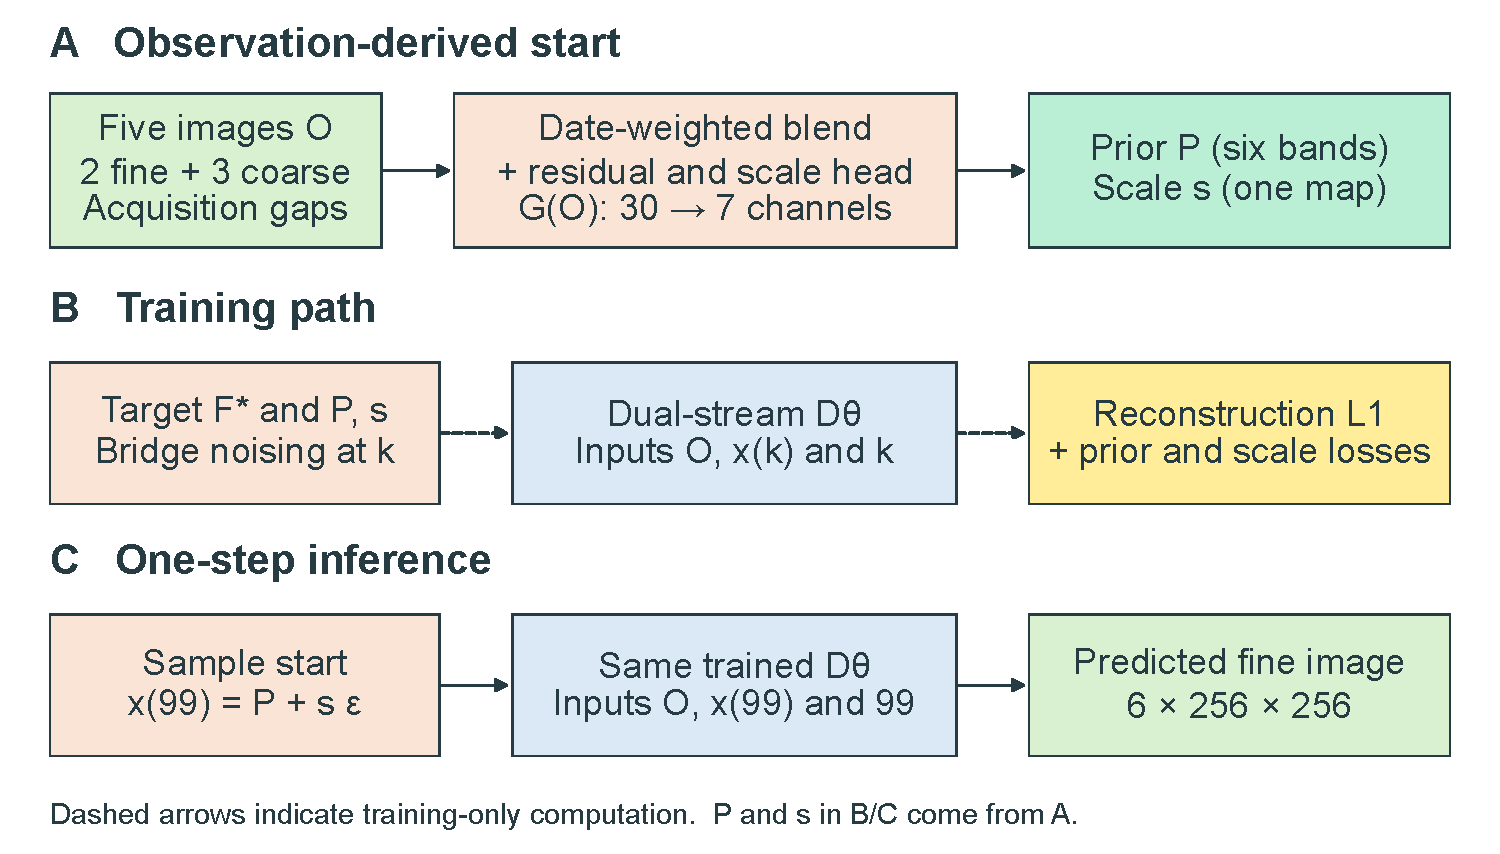
\includegraphics[width=.91\textwidth]{bridge.pdf}
\caption{双锚扩散桥从五幅观测生成均值先验 $P$ 和尺度 $s$。B 区的目标精细影像 $\target$ 用于训练加噪与损失。推理从 $P+s\varepsilon$ 开始并调用一次主干。图中的 $x(k)$ 与 $x(99)$ 对应正文的 $X_k$ 和 $X_{99}$。}
\label{fig:bridge}
\end{figure*}

\subsection{传感器算子对照}
I01 保持高斯起点，在去噪后做两次数据一致性更新。可学习线性算子 $S$ 由各波段归一化的 $5\times5$ 模糊核及行归一化的 $6\times6$ 波段混合矩阵组成。将锚点残差 $C_\pm-S(F_\pm)$ 按日期加权并平滑，得到偏置 $b$。每次更新为
\begin{equation}
Y_{j+1}=Y_j-\lambda S^\top(S(Y_j)+b-C_0),\quad j=0,1 .
\end{equation}
步长 $\lambda$ 通过 sigmoid 限幅。训练还约束两个同日锚的观测残差。这一对照将观测约束放在共享主干的输出端。

\section{实验}
\subsection{数据、训练和评价口径}
实验采用 LGC 影像序列~\cite{emelyanova2013blending}。训练集含十个时序三元组、1,200 个 patch。验证来自一个三元组（2005 年 2 月 14 日、3 月 2 日和 4 月 3 日），含 120 个不重叠 patch。目标日精细影像未出现在训练输入或标签中。该场景曾用于项目开发。本稿冻结相同划分，报告暂停时已完成的单种子（42）基线及七项变体。

各组用 Adam 从零训练 40 轮，每轮 600 次优化器更新。峰值学习率为 $2\times10^{-4}$，先预热 50 步，再以余弦曲线降至峰值的十分之一，梯度范数裁剪阈值为 1。微批次为 1，梯度累积 2 步。在同一训练种子下配对样本次序、共享主干初始化和基础噪声。

验证指标先在反射率域计算各 patch 的 RMSE，再对 120 个 patch 与三组固定推理噪声平均。第 40 轮用当轮训练日志的验证 RMSE。各方法的最佳检查点按 40 轮内最低验证 RMSE 选取，同时报告 SSIM、光谱角 SAM（弧度）、ERGAS（比例 $1/16$）和相关系数 CC。逐块配对时，先对每个 patch 的三次推理取均值。

\subsection{共同终点与最佳检查点}
表~\ref{tab:main} 中，I02 在最佳检查点的平均 RMSE 最低，由基线的 \BaseBest{} 降至 \BridgeBest{}。I01 的相对降幅为 \SensorBestGain\%。I02 的 SAM 与 ERGAS 改善，SSIM 与 CC 略降。统一取第 40 轮时，I02 与 I01 的 RMSE 分别比基线高 \BridgeEndHarm\% 与 \SensorEndHarm\%。在已完成的七个变体中，I03 是唯一第 40 轮 RMSE 低于基线的方案。

I02 的最低验证误差出现在第 9 轮，基线的最低值出现在第 32 轮。图~\ref{fig:curves} 保留了之后的误差变化。此前 14 个方案的六轮共享权重初筛均未超过更强的原始基线门槛。两种训练设置下的排序差异说明，训练配方和检查点规则都需要纳入比较。

\begin{table*}[t]
\centering
\caption{LGC 开发验证结果，含 120 个 patch、一个训练种子（42）及一次去噪主干调用。第 40 轮使用共同终点记录。最佳 RMSE 及其他指标对应各方法最低验证 RMSE 的检查点。改善为相对同种子基线最佳检查点的 RMSE 降幅。}
\label{tab:main}
\setlength{\tabcolsep}{5pt}
\begin{tabular}{lrrrrrrrr}
\toprule
方法 & 第 40 轮 RMSE $\downarrow$ & 最佳轮 & 最佳 RMSE $\downarrow$ & 改善（\%） &
SSIM $\uparrow$ & SAM $\downarrow$ & ERGAS $\downarrow$ & CC $\uparrow$ \\
\midrule
\StageResultRows
\bottomrule
\end{tabular}
\end{table*}

\begin{figure*}[t]
\centering
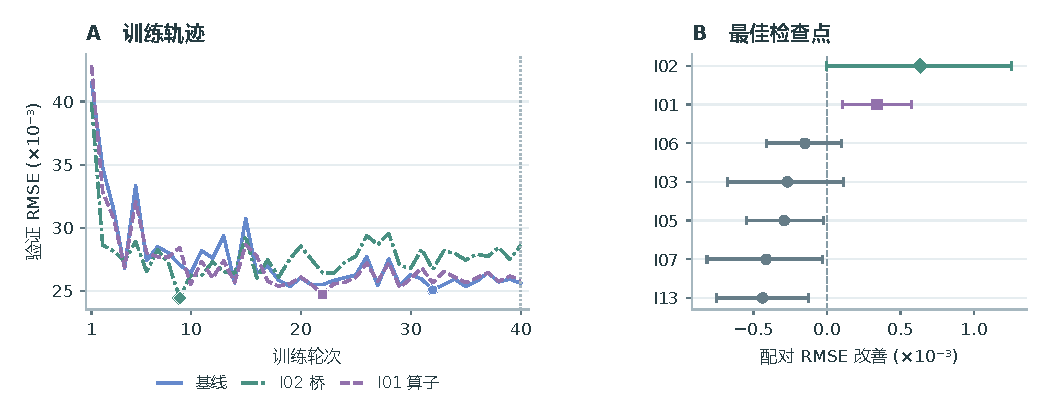
\includegraphics[width=\textwidth]{validation_dynamics_zh.pdf}
\caption{A．验证轨迹，符号为最佳检查点，竖虚线为共同第 40 轮。B．最佳检查点的配对 RMSE 改善定义为基线减变体。点为均值，横线为该场景内 30 个不重叠 $2\times2$ patch 块经 10,000 次有放回重采样后的 2.5 与 97.5 百分位。}
\label{fig:curves}
\end{figure*}

\subsection{双锚桥的改善分布}
最佳检查点下，I02 在 120 个 patch 中改善了 \BridgePatchWins{} 个。平均配对收益为 $\BridgeDiff\times10^{-3}$，空间分块重采样区间为 $[\BridgeLower,\BridgeUpper]\times10^{-3}$，包含零。该区间描述已训练模型在单场景内的空间波动，训练种子与日期间变异需要其他复验。

为分析空间差异，用反射率域的粗观测 $C_0$ 与插值 $(1-w)C_-+wC_+$ 的平均绝对差对 patch 排序，划分每组 40 块的三分位。由低到高的相对 RMSE 改善分别为 \BridgeLow\%、\BridgeMid\% 和 \BridgeHigh\%（图~\ref{fig:strata}）。平均收益集中在目标粗观测较接近参考插值的区域。

\begin{figure}[!t]
\centering
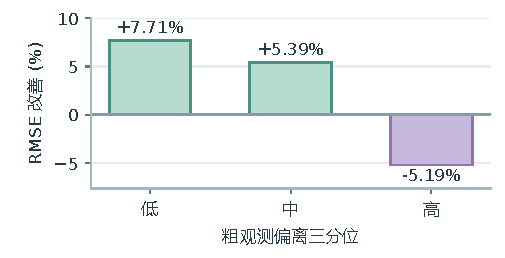
\includegraphics[width=\columnwidth]{coarse_strata_zh.pdf}
\caption{I02 在粗观测偏离程度三分位上相对于基线的 RMSE 改善，按各方法最佳检查点计算，每组 40 个 patch。分组为事后分析，反映目标粗观测与参考插值的接近程度。}
\label{fig:strata}
\end{figure}

\section{讨论与结论}
双锚扩散桥在较早轮次取得较低验证误差，而在共同终点的误差较高。选模规则因此会影响对单步融合性能的判断。高偏离组的结果提示插值先验可能在这类区域作用较弱。粗观测差异也会受到传感器和其他观测因素影响，暂不能归因到真实地物变化。I02 同时引入了先验、尺度和辅助损失，对应的独立贡献仍待区分。

I01 在去噪后约束观测一致性，提供了另一种作用位置。考察两项机制时，都需要保留学习轨迹及相同训练预算下的对照。本稿冻结了单种子、单验证日期的阶段结果。多种子、独立 LGC 场景与 Coleambally Irrigation Area（CIA）可用于检验稳定性及迁移。外部强方法需要统一评测和训练口径。SA-STF 作者训练划分中含本稿验证日期 2005 年 3 月 2 日~\cite{zhang2026sastf}。

\textbf{可复算材料。} 阶段包包含冻结清单、运行配置、40 轮日志、配对 patch 指标及绘图源码，可据此复算稿中数值。

\bibliographystyle{IEEEbib}
\bibliography{refs}
\end{document}
